\documentclass[12pt]{article}
\usepackage{graphicx}
\usepackage{amsmath}
\usepackage{mathtools}
\usepackage{gensymb}

\newcommand{\mydet}[1]{\ensuremath{\begin{vmatrix}#1\end{vmatrix}}}
\providecommand{\brak}[1]{\ensuremath{\left(#1\right)}}
\providecommand{\norm}[1]{\left\lVert#1\right\rVert}
\newcommand{\solution}{\noindent \textbf{Solution: }}
\newcommand{\myvec}[1]{\ensuremath{\begin{pmatrix}#1\end{pmatrix}}}
\let\vec\mathbf

\begin{document}
\begin{center}
\textbf\large{CHAPTER-7 \\ COORDINATE GEOMETRY}

\end{center}
\section*{Excercise 7.1}

Q6.Name the type of quadilateral formed,if any, by the following points, and give reasons for your answer:
\begin{enumerate}
	\item $\brak{-1,-2}, \brak{1,0}, \brak{-1,2}, \brak{-3,0}$ 
	\item $\brak{-3,5}, \brak{3,1}, \brak{0,3}, \brak{-1,-4}$
	\item $\brak{4,5}, \brak{7,6}, \brak{4,3}, \brak{1,2}$
\end{enumerate}
\solution
\begin{enumerate}
\item The coordinates are given as
	\begin{align}
	\vec{A} = \myvec{
		-1\\
		-2\\
		},
	\vec{B} = \myvec{
		1\\
		0\\
		},
	\vec{C} = \myvec{
		-1\\
		2\\
		} \text{ and }
	\vec{D} = \myvec{
		-3\\
		0\\
		}
	\end{align}
	\begin{align}
		\vec{B} - \vec{A} &= \myvec{1\\0} - \myvec{-1\\-2} = \myvec{2\\2}\\
		\vec{C} - \vec{B} &= \myvec{-1\\2} - \myvec{1\\0} = \myvec{-2\\2}\\
		\vec{C} - \vec{D} &= \myvec{-1\\2} - \myvec{-3\\0} = \myvec{2\\2}\\
		\vec{D} - \vec{A} &= \myvec{-3\\0} - \myvec{-1\\-2} = \myvec{-2\\2}\\
		\vec{C} - \vec{A} &= \myvec{-1\\2} - \myvec{-1\\-2} = \myvec{0\\4}\\
		\vec{D} - \vec{B} &= \myvec{-3\\0} - \myvec{1\\0} = \myvec{-4\\0}
	\end{align}
	\begin{align}	
		\vec{B}-\vec{A} = \vec{C}-\vec{D} \text{ and } \vec{C}-\vec{B} = \vec{D}-\vec{A}.
	\end{align}
	Hence, $ABCD$ is a parallelogram.
	\begin{enumerate}
		\item Now checking if the adjacent sides are orthogonal to each other
	\begin{align}
		(\vec{B}-\vec{A})^\top (\vec{C}-\vec{B}) = \myvec{2&2} \myvec{-2\\2} = -4+4 = 0
	\end{align}
		\item Now checking if the diagonals are also orthogonal then it is a square else a rectangle.
	\end{enumerate}	
	\begin{align}
		(\vec{C}-\vec{A})^\top (\vec{D}-\vec{B}) = \myvec{0&4} \myvec{-4\\0} = 0
	\end{align}
	Hence the diagonals are orthogonal to each other.

	So, we can conclude that $ABCD$ is a square.

	As shown in Figure \ref{fig:Fig1} we can see that $ABCD$ is a square hence we can conclude that our theoritical result is verified.
 
\begin{figure}[!h]
	\begin{center} 
	    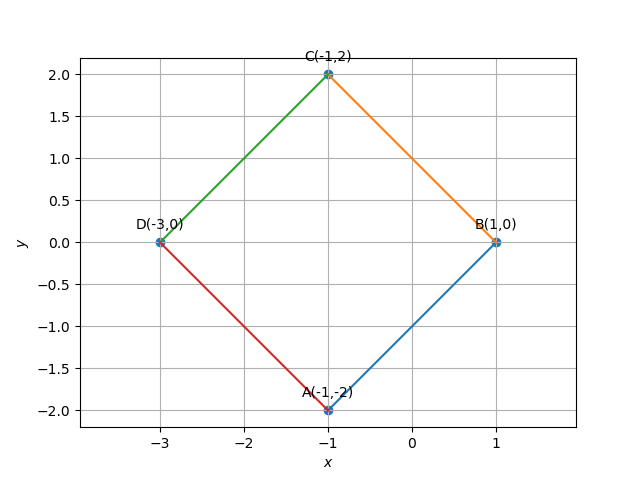
\includegraphics[width=\columnwidth]{figs/quad1}
	\end{center}
\caption{}
\label{fig:Fig1}
\end{figure}

\item The coordinates are given as
	\begin{align}
	\vec{A} = \myvec{
		-3\\
		5\\
		},
	\vec{B} = \myvec{
		3\\
		1\\
		},
	\vec{C} = \myvec{
		0\\
		3\\
		} \text{ and }
	\vec{D} = \myvec{
		-1\\
		-4\\
		}
	\end{align}
	\begin{align}
		\vec{B} - \vec{A} &= \myvec{3\\1} - \myvec{-3\\5} = \myvec{6\\-4}\\
		\vec{C} - \vec{B} &= \myvec{0\\3} - \myvec{3\\1} = \myvec{-3\\2}\\
		\vec{C} - \vec{D} &= \myvec{0\\3} - \myvec{-1\\-4} = \myvec{1\\7}\\
		\vec{D} - \vec{A} &= \myvec{-1\\-4} - \myvec{-3\\5} = \myvec{2\\-9}\\
		\vec{C} - \vec{A} &= \myvec{0\\3} - \myvec{-3\\5} = \myvec{3\\-2}\\
		\vec{D} - \vec{B} &= \myvec{-1\\-4} - \myvec{3\\1} = \myvec{-4\\-5}
	\end{align}
	\begin{align}
	\vec{B}-\vec{A} \neq \vec{C}-\vec{D} \text{ and } \vec{C}-\vec{B} \neq \vec{D}-\vec{A},
	\end{align}
	Hence, $ABCD$ is not a parallelogram, it can be a irregular quadilateral.
	\begin{enumerate}
		\item Now to check if any three points are collinear,

	if rank of $\myvec{\vec{B}-\vec{A} & \vec{C}-\vec{B}} = 1$ then points are collinear

	Forming the collinearity matrix
	\begin{align}
		\myvec{6&-3\\-4&2} \xleftrightarrow{R_{2}\rightarrow R_{2}+\frac{2}{3}R_{1}}= \myvec{6&-3\\0&0}
	\end{align}
	\end{enumerate}
	Hence, rank = 1

	Since none of the opposite sides are parallel to each other and three points are collinear so these does not form a quadilateral.

	As shown in Figure \ref{fig:Fig2} we can see that $ABCD$ does not form a quadilateral and three points are collinear hence, our theoritical result is verified.
	
\begin{figure}[!h]
	\begin{center} 
	    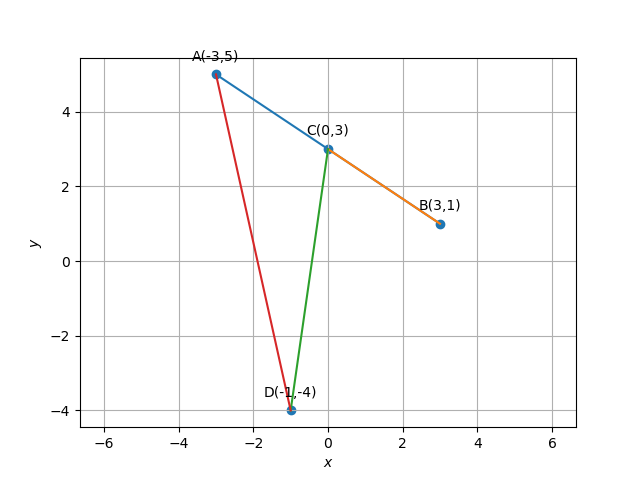
\includegraphics[width=\columnwidth]{figs/quad2}
	\end{center}
\caption{}
\label{fig:Fig2}
\end{figure}
	
\item The coordinates are given as
	\begin{align}
	\vec{A} = \myvec{
		4\\
		5\\
		},
	\vec{B} = \myvec{
		7\\
		6\\
		},
	\vec{C} = \myvec{
		4\\
		3\\
		} \text{ and }
	\vec{D} = \myvec{
		1\\
		2\\
		}
	\end{align}
	\begin{align}
		\vec{B} - \vec{A} &= \myvec{7\\6} - \myvec{4\\5} = \myvec{3\\1}\\
		\vec{C} - \vec{B} &= \myvec{4\\3} - \myvec{7\\6} = \myvec{-3\\-3}\\
		\vec{C} - \vec{D} &= \myvec{4\\3} - \myvec{1\\2} = \myvec{3\\1}\\
		\vec{D} - \vec{A} &= \myvec{1\\2} - \myvec{4\\5} = \myvec{-3\\-3}\\
		\vec{C} - \vec{A} &= \myvec{4\\3} - \myvec{4\\5} = \myvec{0\\-2}\\
		\vec{D} - \vec{B} &= \myvec{1\\2} - \myvec{7\\6} = \myvec{-6\\-4}\\
	\end{align}
	\begin{align}
		\vec{B}-\vec{A} = \vec{C}-\vec{D} \text{ and } \vec{C}-\vec{B} = \vec{D}-\vec{A},
	\end{align}
	Hence, $ABCD$ is a parallelogram.
	\begin{enumerate}
		\item Now checking if the adjacent sides are orthogonal to each other
	\begin{align}
		(\vec{B}-\vec{A})^\top (\vec{C}-\vec{B}) = \myvec{3&1} \myvec{-3\\-3} = -9-3 = -12
	\end{align}
	Since inner product is not zero so adjacent sides are not orthogonal.

	Hence, we can say that $ABCD$ is neither a rectangle nor a square.

		\item Now checking if the diagonals are orthogonal then it is a Rhombus.
	\begin{align}
		(\vec{C}- \vec{A})^\top (\vec{D}-\vec{B}) = \myvec{0&-2} \myvec{-6\\-4} = 0+8 = 8
	\end{align}
	\end{enumerate}		
	Hence the diagonals are also not orthogonal so we conclude that $ABCD$ is a parallelogram.

	As shown in Figure \ref{fig:Fig3} we can see that $ABCD$ forms a parallelogram hence, our theoritical result is verified.

\begin{figure}[!h]
	\begin{center} 
	    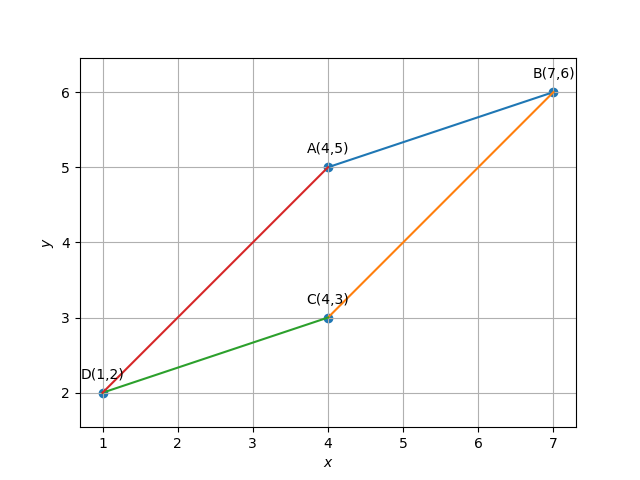
\includegraphics[width=\columnwidth]{figs/quad3}
	\end{center}
\caption{}
\label{fig:Fig3}
\end{figure}
\end{enumerate}

\end{document}

